\documentclass[a4paper,11pt]{article}
\usepackage[utf8]{inputenc}
\usepackage[russian]{babel}
\usepackage[T1]{fontenc}
\usepackage{amssymb,amsmath,graphicx,clrscode,indentfirst}

\author{Иван Веселов}
\title{Курс kiev-clrs -- Лекция 16. Жадные алгоритмы. Графы.}
\date{2009 г.}

\begin{document}

\maketitle
\tableofcontents
\newpage

\setlength{\parskip}{1ex plus 0.5ex minus 0.2ex}

\section{План лекции}
\begin{itemize}
\item Представление графов
\item Минимальные остовные деревья
\item Оптимальная подструктура
\item Жадный выбор
\item Алгоритм Прима
\end{itemize}

\section{Графы}

\textbf{Ориентированный граф} (орграф) $G = (V, E)$ -- это упорядоченная пара,
состоящая из множества вершин $V$ и множества рёбер $E \subseteq V \times V$

В неориентированном графе $G = (V, E)$, множество рёбер $E$ состоит из
\emph{неупорядоченных} пар вершин.

В любом случае получаем $|E| = O(V^2)$.

Кроме того, если граф $G$ связен, то $ |E| \geqslant |V| - 1$, таким образом получаем, что
$\lg |E| = \Theta(\lg V)$.

\textbf{Матрица инцидентности} для графа $G = (V, E)$, где $V = 1, 2, \cdots, n$:

$$
A[i, j] = \begin{cases}
  1 \text{ если } (i, j) \in E \\
  0 \text{ в противном случае}
\end{cases}
$$

\begin{figure}[ht]
  \centering
  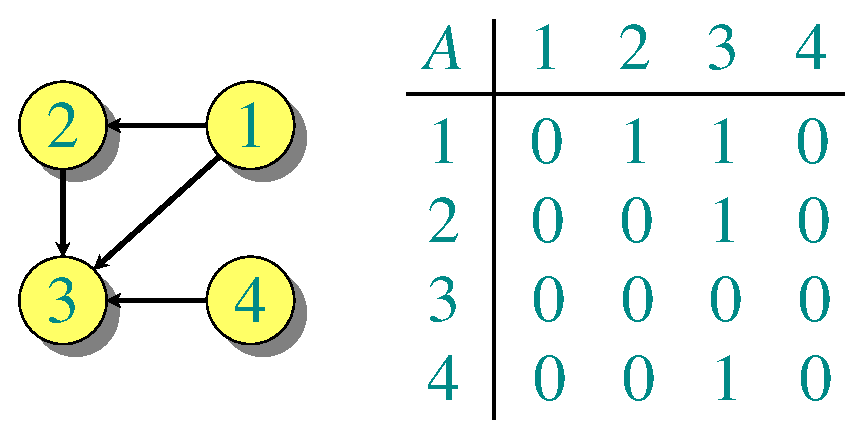
\includegraphics[width=3in]{lecture16/adjacency-matrix.eps}
  \caption{Матрица инцидентности}
  \label{fig:adjacency}
\end{figure}

Это так называемое плотное заполнениие. Для разреженных матриц больше подходит
списочное представление графа. Т.е. для каждой вершины $v$ -- имеем список
вершин $Adj[v]$, который задаётся исходящими из вершины $v$ рёбрами.

\begin{gather*}
Adj[1] = \{ 2, 3 \} \\
Adj[2] = \{ 3 \} \\
Adj[3] = \{ \} \\
Adj[4] = \{ 3 \} 
\end{gather*}

Для ориентированных графов размер этого списка называется ``исходящей степенью''
вершины.

Для неориентированных графов -- просто ``степенью''.

Лемма о рукопожатиях:

$\sum_{ v \in V}{degree(v)} = 2|E| $ для неориентированного графа, таким образом
списки смежности используют $\Theta(V + E)$ места для хранения.

\section{Минимальные остовные деревья}
Вход: взвешенный связный неориентированный граф $G = (V, E)$ c функцией веса $W
\colon E \to \mathbb{R}$

Для простоты предположим, что все веса различны.

Результат: остовное дерево $T$, которое соединяет все вершины и обладает минимальным
весом

$$
w(T) = \sum_{(u,v) \in T} w(u, v)
$$

\begin{figure}[ht]
  \centering
  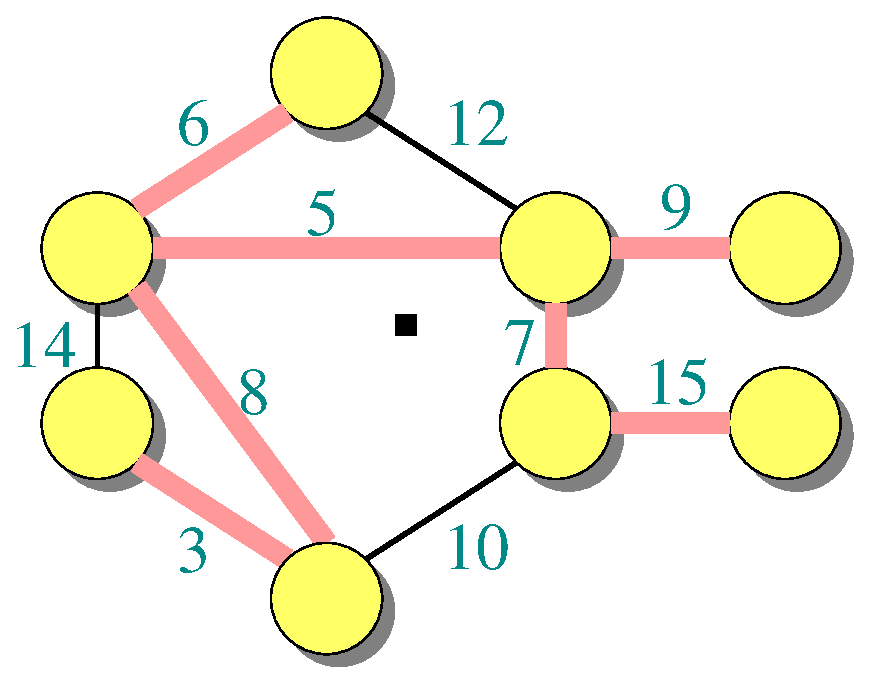
\includegraphics[width=3in]{lecture16/graph-mst.eps}
  \caption{Минимальное остовное дерево}
  \label{fig:mst}
\end{figure}

Оптимальная подструктура.

Рассмотрим минимальное остовное дерево $T$, без указания всего остального графа
$G$.

\begin{figure}[ht]
  \centering
  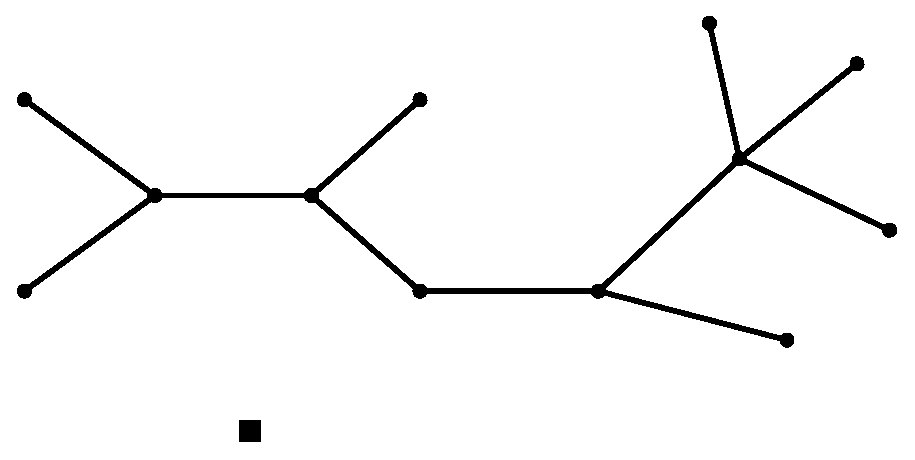
\includegraphics[width=3in]{lecture16/mst1.eps}
  \caption{Минимальное остовное дерево}
  \label{fig:mst1}
\end{figure}

Рассмотрим какое-либо ребро $(u, v)$ 

\begin{figure}[ht]
  \centering
  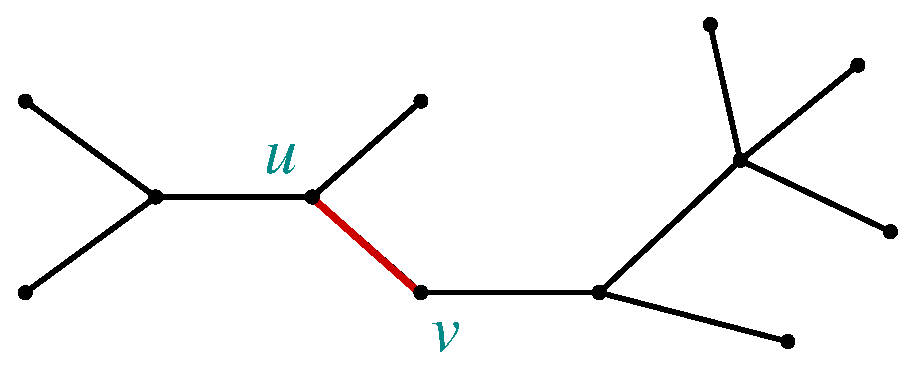
\includegraphics[width=3in]{lecture16/mst2.eps}
  \caption{Минимальное остовное дерево -- с выделенным ребром $(u, v)$}
  \label{fig:mst2}
\end{figure}

и удалим его

\begin{figure}[ht]
  \centering
  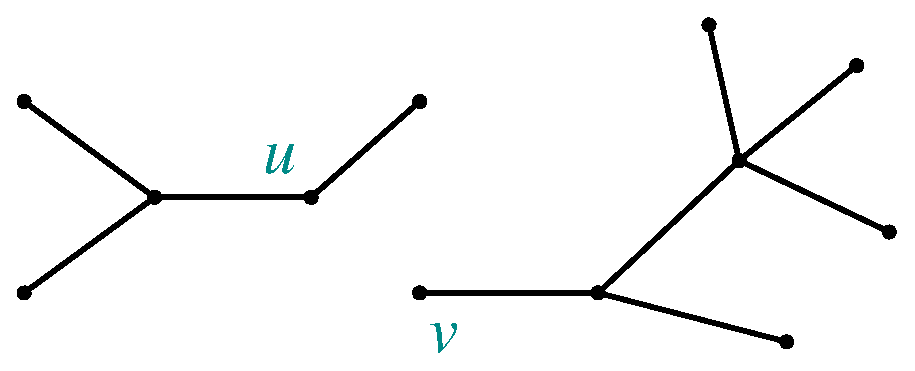
\includegraphics[width=3in]{lecture16/mst3.eps}
  \caption{Минимальное остовное дерево -- после удаления ребра}
  \label{fig:mst3}
\end{figure}

После этого дерево перестанет быть связным и распадётся на два поддерева

\begin{figure}[ht]
  \centering
  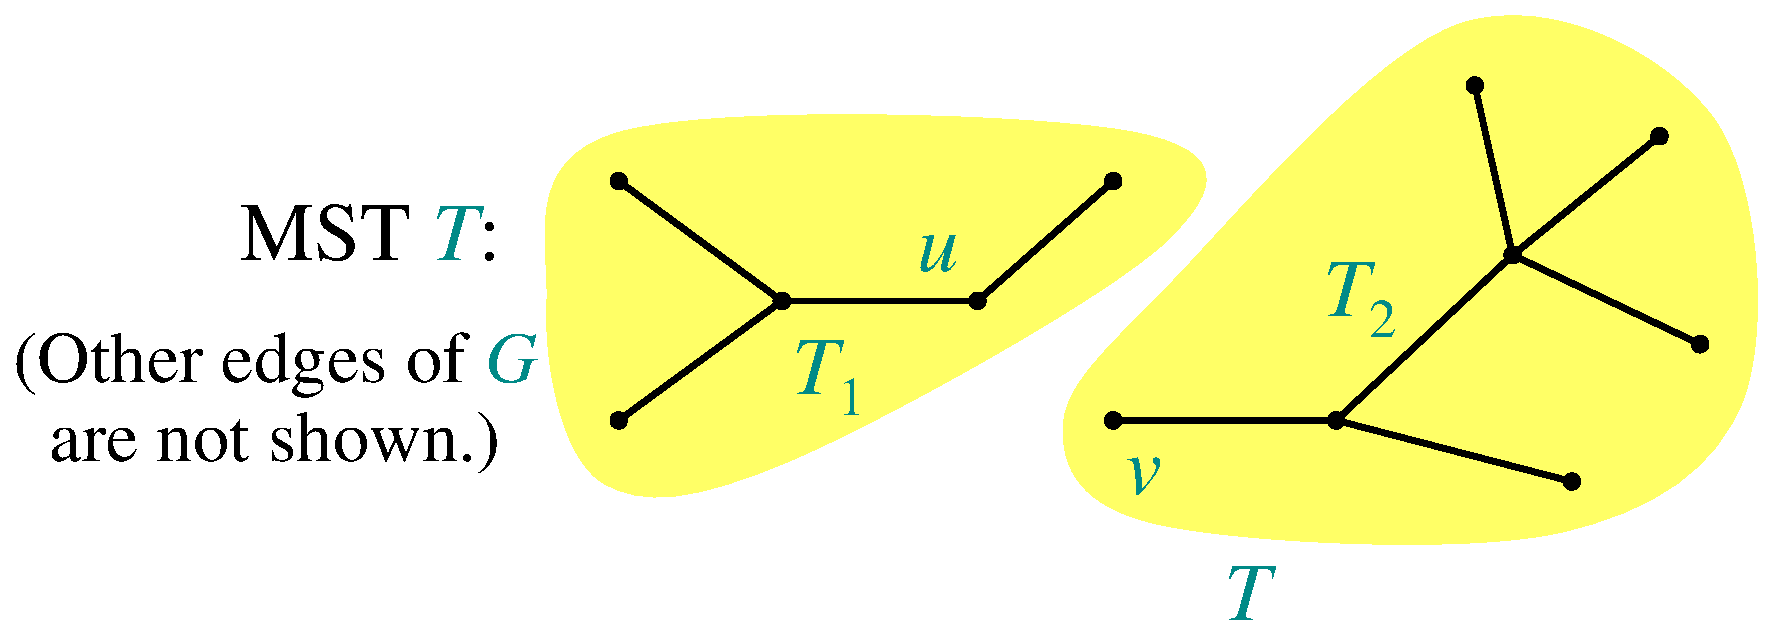
\includegraphics[width=3.5in]{lecture16/mst4.eps}
  \caption{Минимальное остовное дерево с двумя поддеревьями}
  \label{fig:mst4}
\end{figure}

О том, что имеет место оптимальная подструктура говорит следующая \textbf{теорема}:

Поддерево $T_1$, являеется МОД для графа $G_1 = (V_1, E_1)$, который является
подграфом $G$ и индуцирован по вершинам $T_1$, то есть включает в себя только те
рёбра, что соединяют вершины $V_1$. Более формально:

\begin{gather*}
  V_1 = \text{вершины } T_1 \\
  E_1 = \{ (x, y) \in E \colon x, y \in E_1 \}
\end{gather*}


Аналогично для $T_2$.

\textbf{Доказательство} (техника ``Cut and paste'')

Вес МОД $T$:
$$
w(T) = w(T_1) + w(u,v)+ w(T2)
$$

Пусть $T_1'$ -- является ОД для графа $G_1$ с меньшим весом чем $T_1$ Тогда мы
могли бы использовать (``вставить'') его в нашем оригинальном дереве $T$ и
получить вес

$$
w'(T) = w(T_1') + w(u,v)+ w(T2) < w(T)
$$

что противоречит изначальному предположению о том, что $w(t)$ -- минимален.

Получается, что у нас есть оптимальная подструктура. Есть ли пересекающиеся
подзадачи? Да, т.к. нам приходится несколько раз решать одну и ту же подзадачу
для какой-то части графа.

Значит мы можем использовать динамическое программирование!

Но кроме это у нашей задачи есть ещё одно важное свойство, которое позволяет
решить задачу эффективнее.

\textbf{Признак жадного алгоритма}

\emph{Свойство жадного выбора} -- означает, что локально оптимальный выбор является и
глобально оптимальным.

О том, что для МОД выполняется свойство жадного выбора говорит следующая
\textbf{теорема}:

Пусть $T$ -- МОД для $G = (V, E)$ и пусть $A \subseteq V$. Предположим, что $(u,
v) \in E$ -- ребро с наименьшим весом среди рёбер соединяющих $A$ с $V - A$.
Тогда $(u, v) \in T$

\begin{figure}[ht]
  \centering
  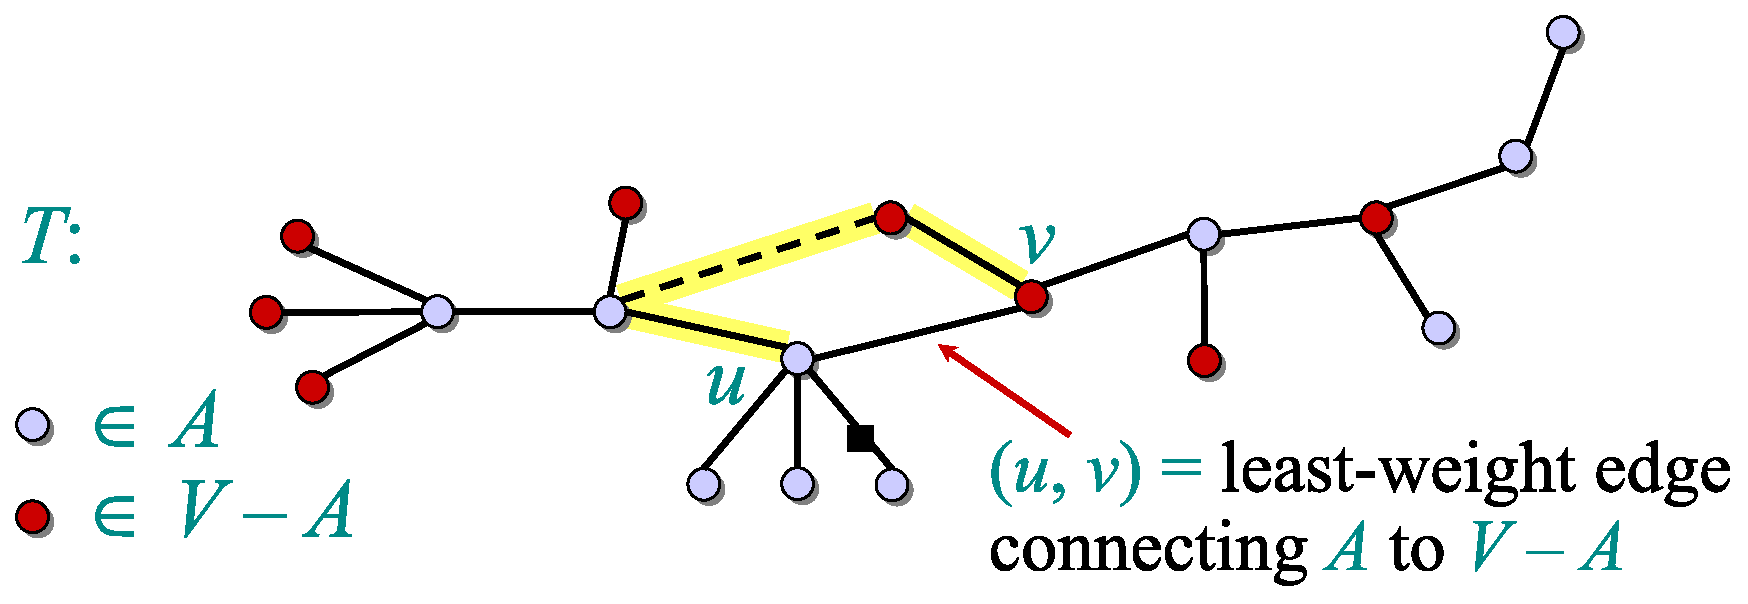
\includegraphics[width=4in]{lecture16/mst-proof.eps}
  \caption{Иллюстрация доказательства}
  \label{fig:mst-proof}
\end{figure}

\textbf{Доказательство} (``cut and paste'')
\begin{itemize}
  
\item пусть ребро $(u, v) \notin T$ и является ребром с наименьшим весом среди тех,
что соединяют $A$ и $V-A$.
\item заметим, что должен существовать единый простой путь от $u$ к $v$ в нашем
  МОД $T$
\item заменим $(u, v)$ на первое ребро этого пути, которое соединяет $A$ и $V -
  A$ (такое ребро всегда есть, т.к. $u$ и $v$ находятся в разных множествах и
  где-то должен быть переход).
\item получим МОД с меньшим суммарным весом, что ведёт к противоречию
\end{itemize}

\section{Алгоритм Прима}

Идея: представить $V - A$ c помощью очереди с приоритетами $Q$. Каждая вершина в
$Q$ будет хранить ключ -- значение наименьшего по весу ребра, соединяющего её с
вершинами из $A$.

\begin{codebox}
\li $Q \gets V $
\li $key[v] \gets \infty$ для всех $v \in V$
\li $key[s] \gets 0$ для некоего $s \in V$
\li \While $Q \neq \emptyset$
\li \Do $u \gets \proc{Extract-Min}(Q)$
\li \For each $v \in Adj[u]$
\li \Do \If $v \in Q$ и $w(u, v) < key(v)$
\li \Then $key[v] \gets w(u,v)$
\li $\pi(v) \gets u$
  \End
  \End
  \End
\end{codebox}

В конце возвращаем $\{ (v, \pi(v))\}$

\begin{figure}[ht]
  \centering
  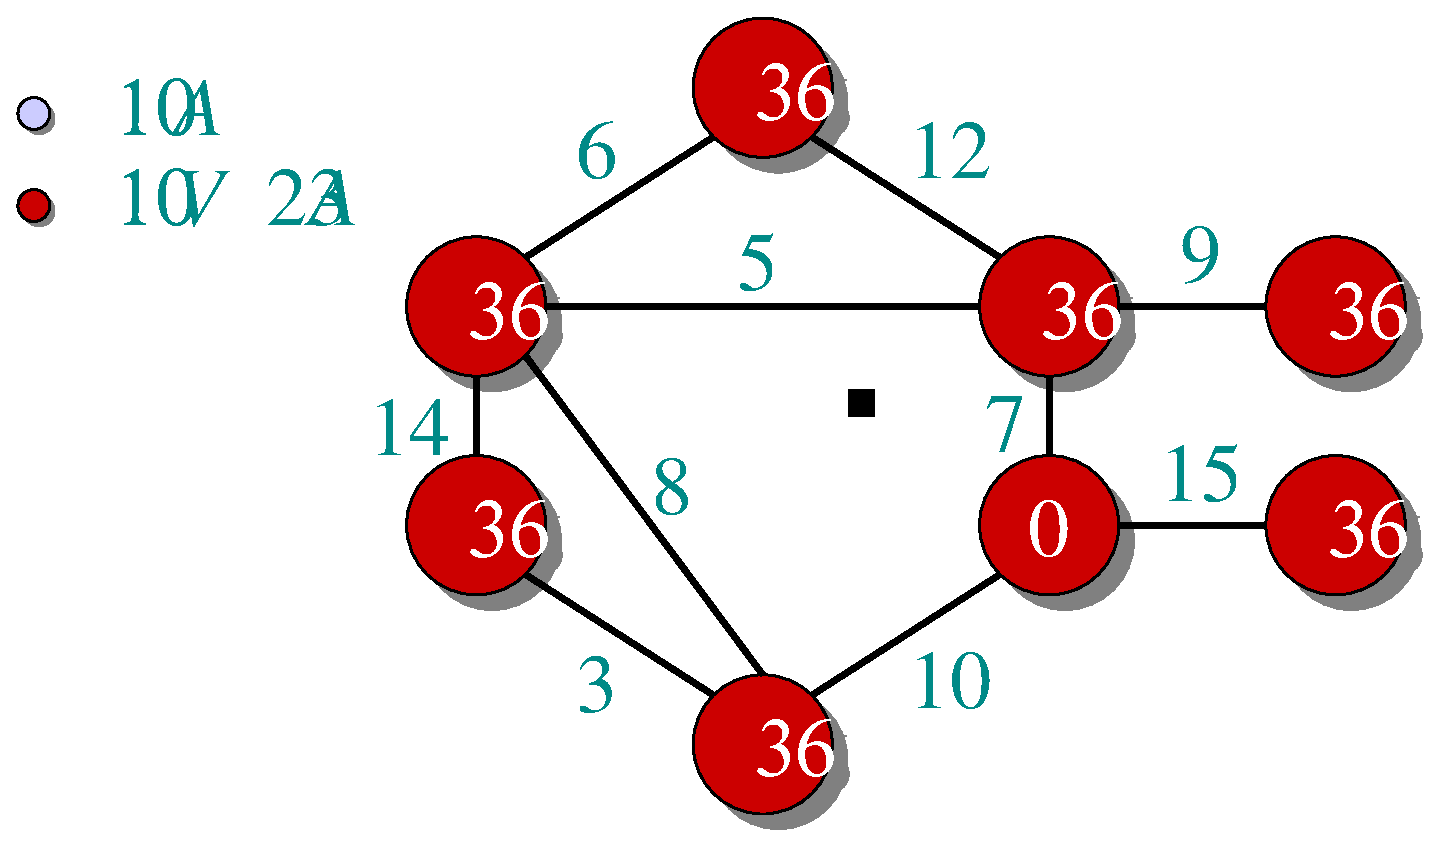
\includegraphics[width=4in]{lecture16/prim1.eps}
  \caption{Пример алгоритма Прима}
\end{figure}

\begin{figure}[ht]
  \centering
  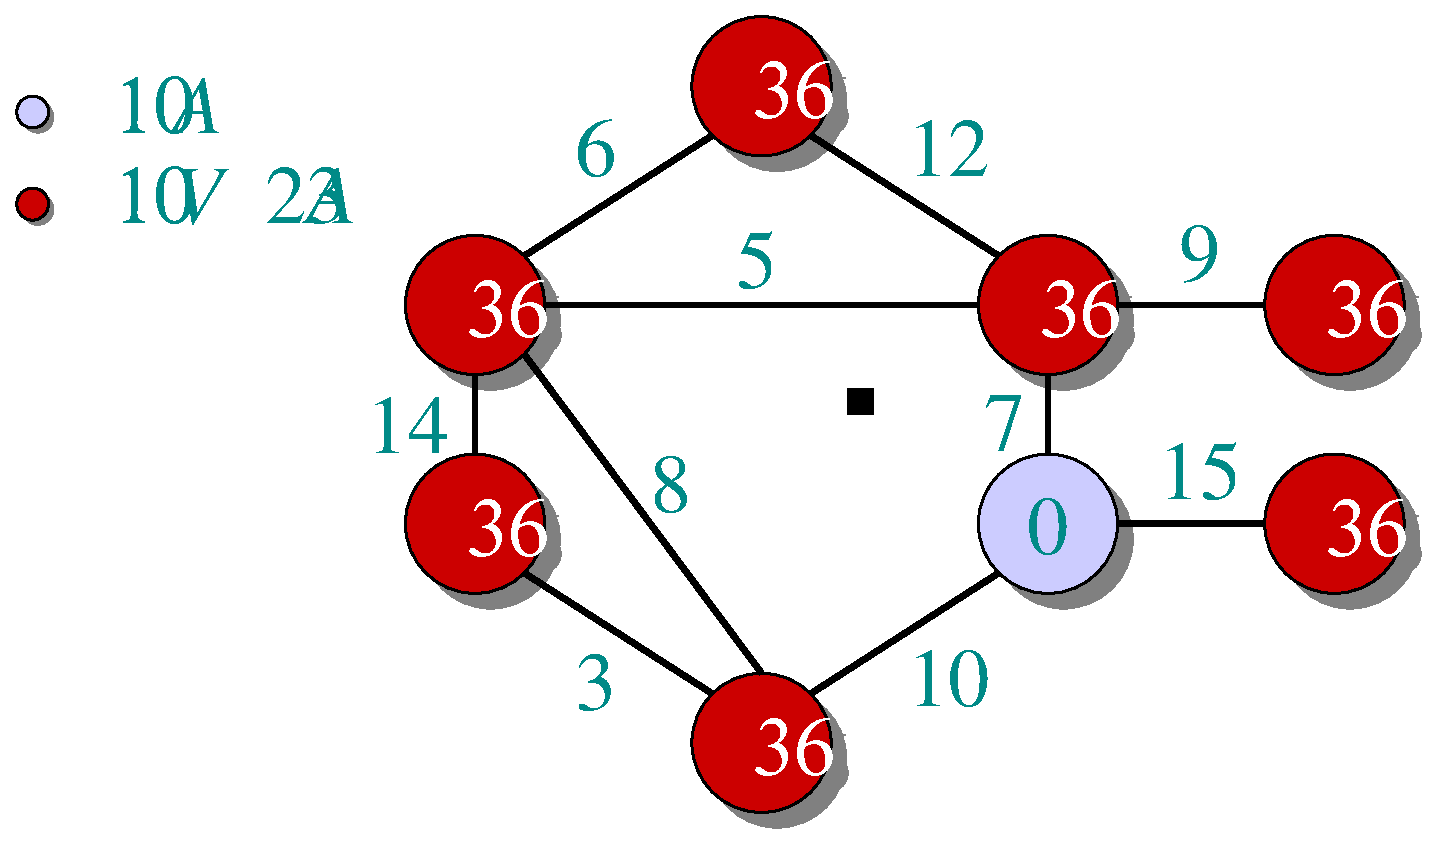
\includegraphics[width=4in]{lecture16/prim2.eps}
  \caption{Пример алгоритма Прима}
\end{figure}
\begin{figure}[ht]
  \centering
  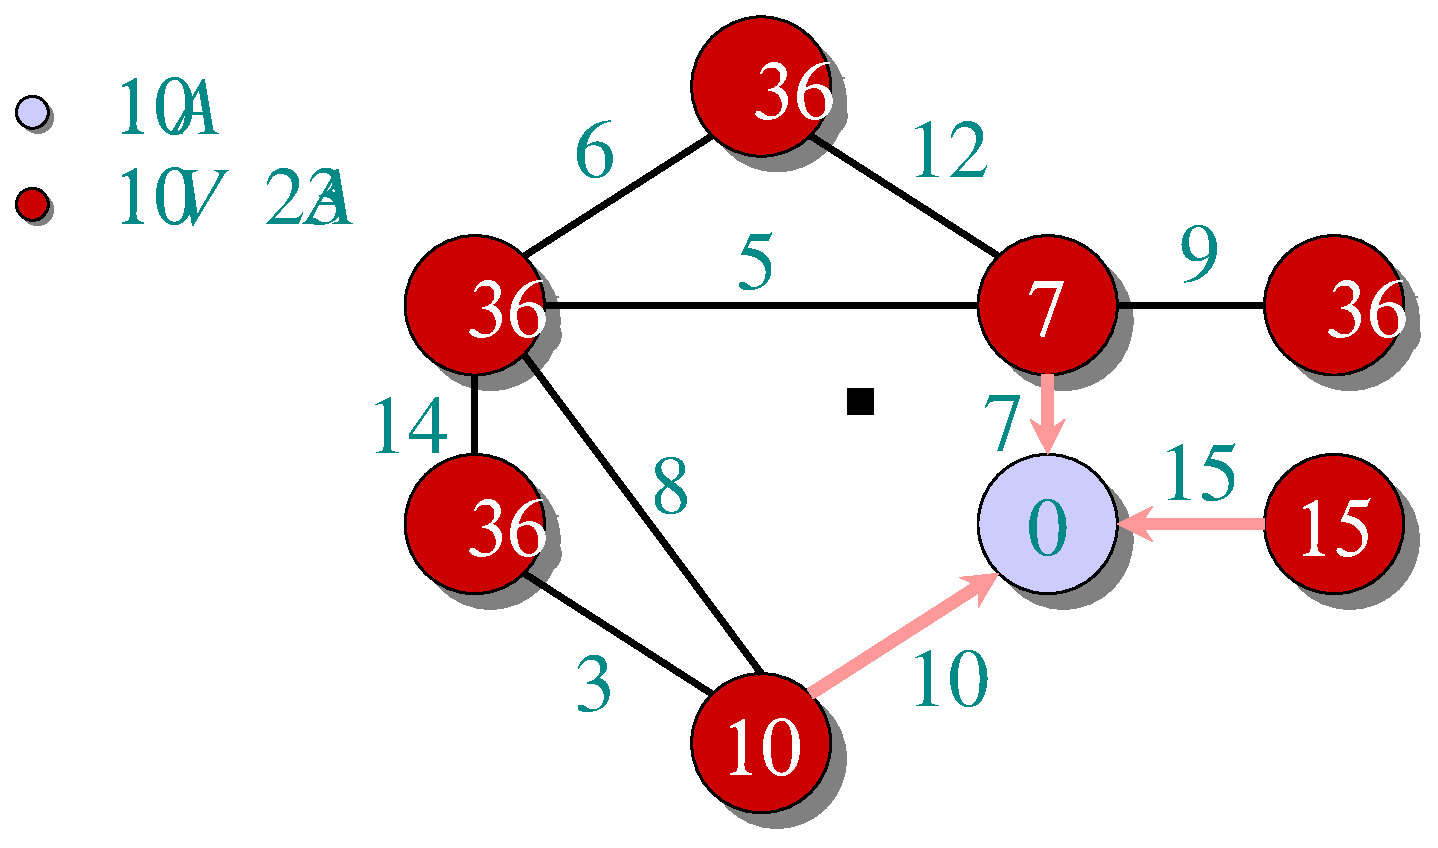
\includegraphics[width=4in]{lecture16/prim3.eps}
  \caption{Пример алгоритма Прима}
\end{figure}
\begin{figure}[ht]
  \centering
  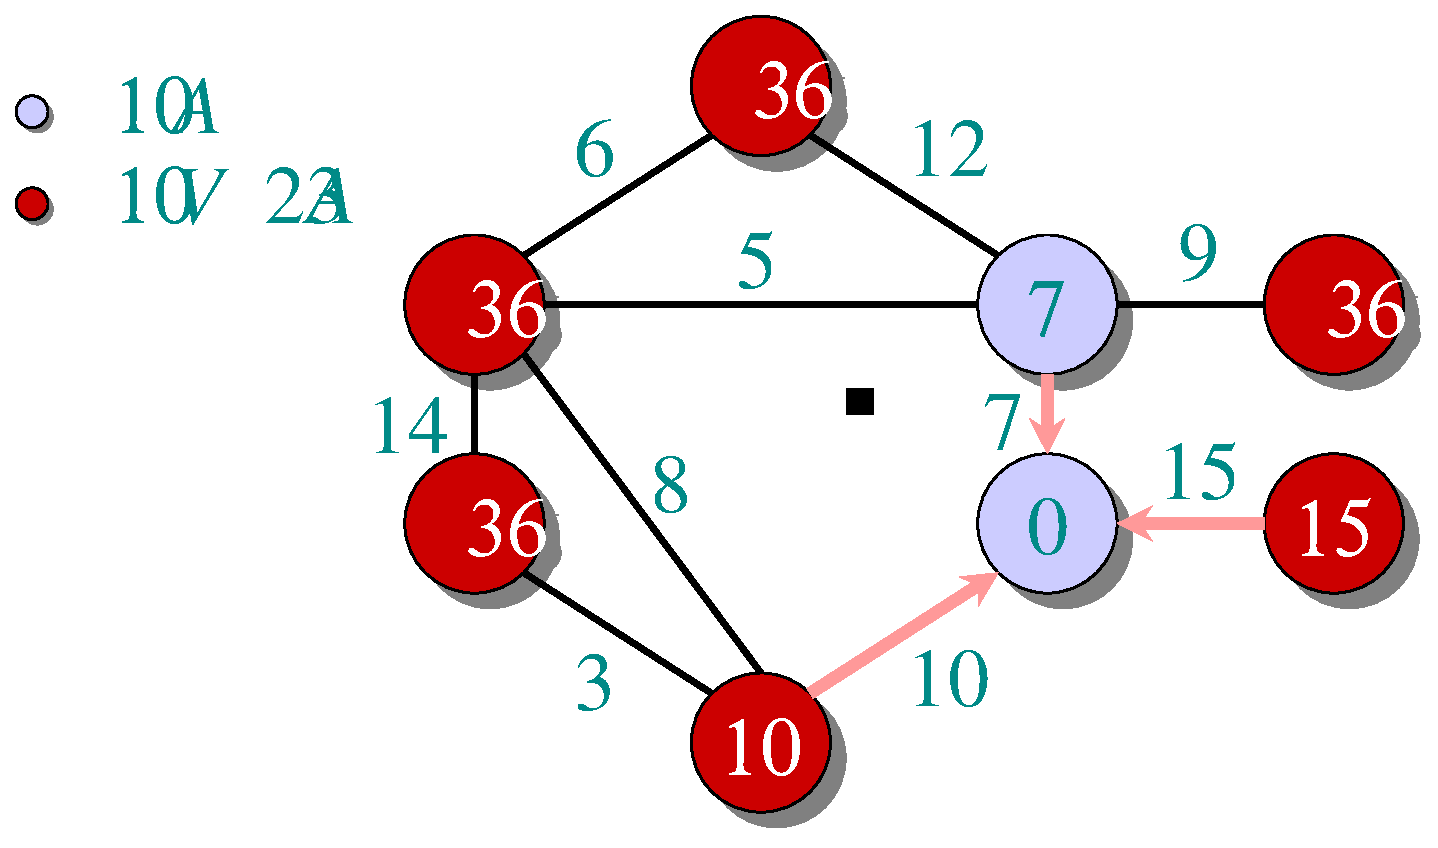
\includegraphics[width=4in]{lecture16/prim4.eps}
  \caption{Пример алгоритма Прима}
\end{figure}
\begin{figure}[ht]
  \centering
  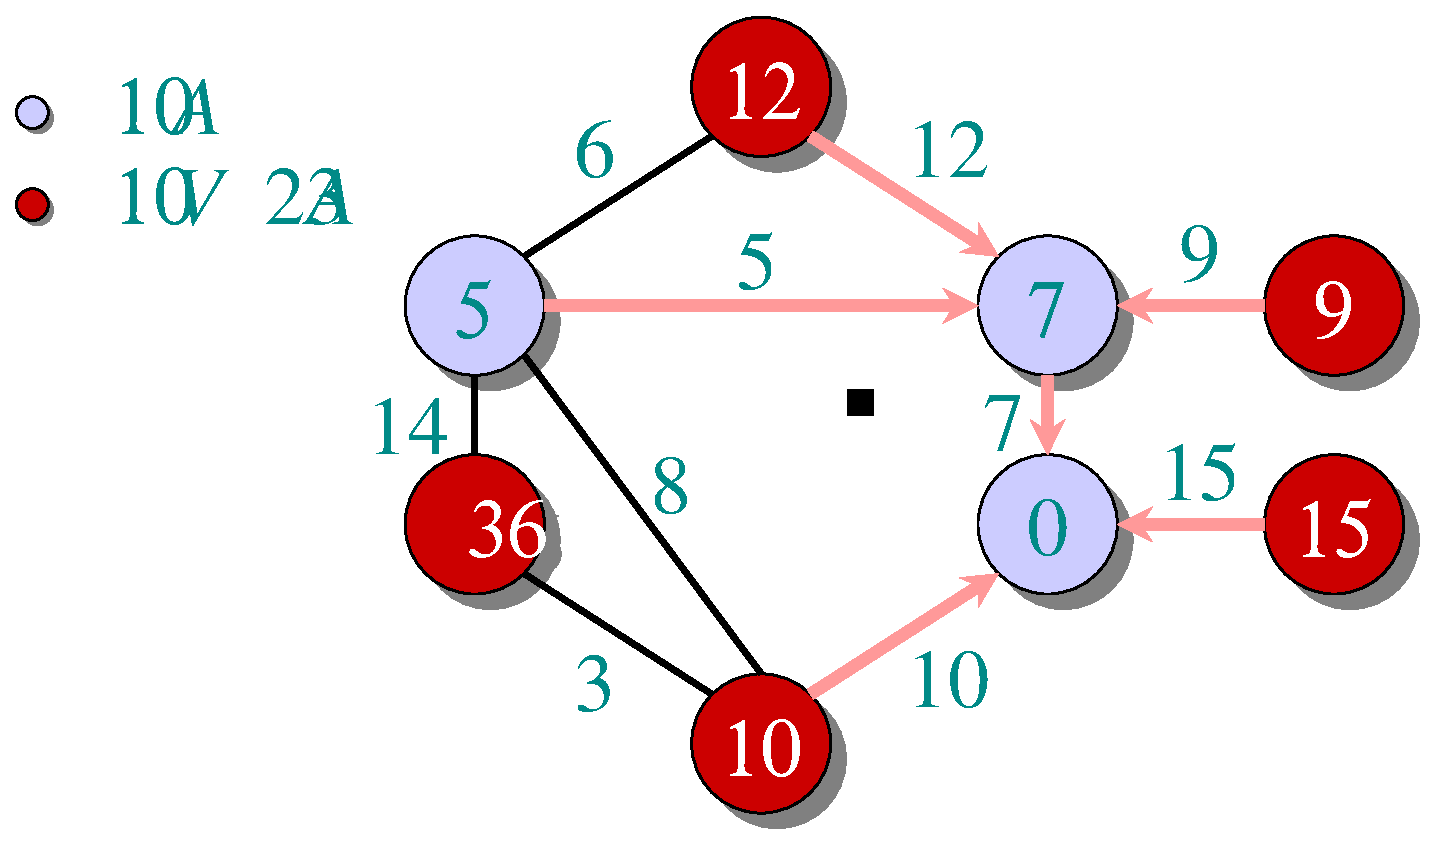
\includegraphics[width=4in]{lecture16/prim6.eps}
  \caption{Пример алгоритма Прима}
\end{figure}
\begin{figure}[ht]
  \centering
  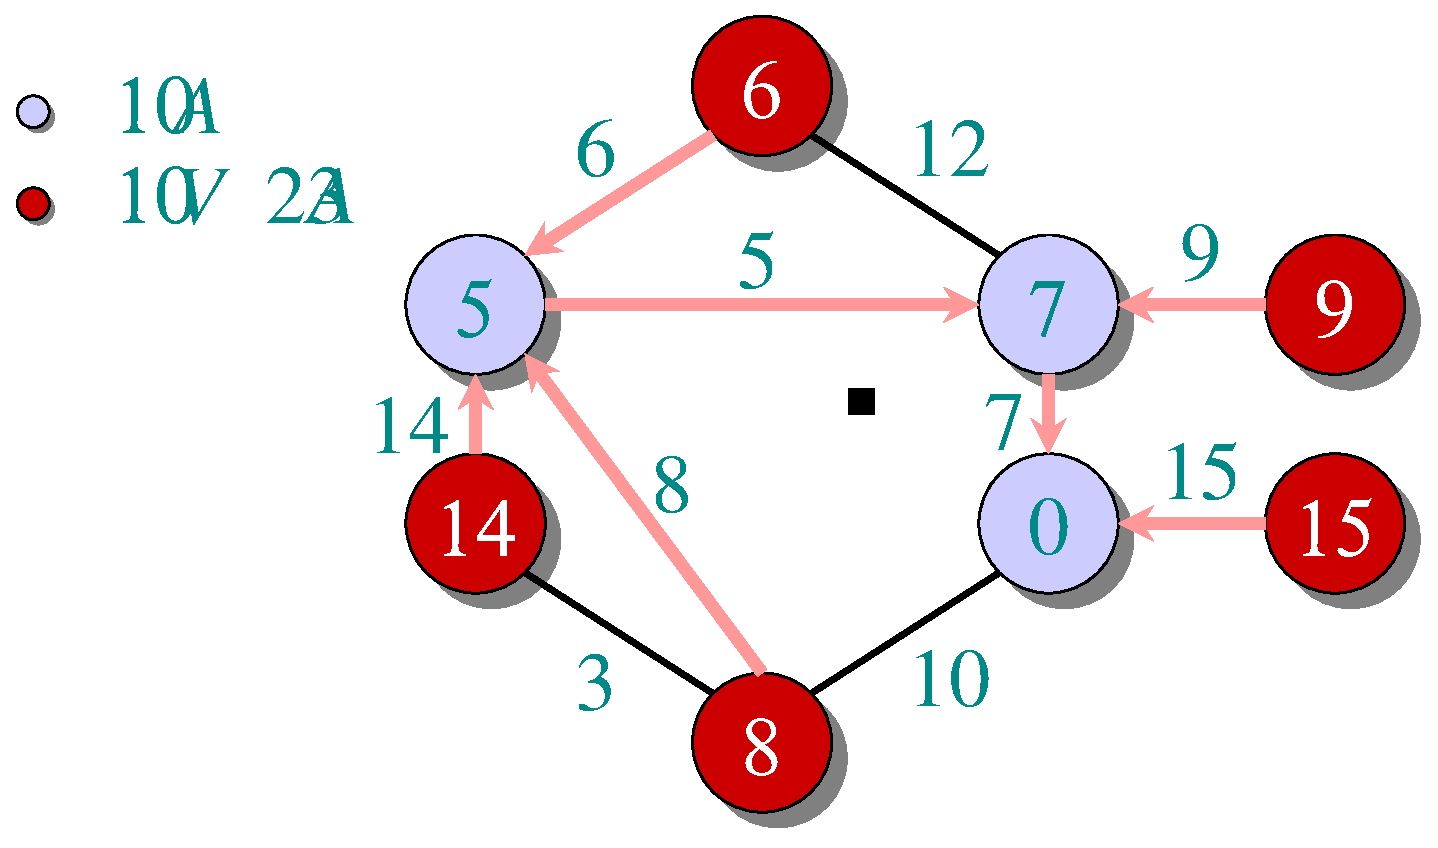
\includegraphics[width=4in]{lecture16/prim7.eps}
  \caption{Пример алгоритма Прима}
\end{figure}
\begin{figure}[ht]
  \centering
  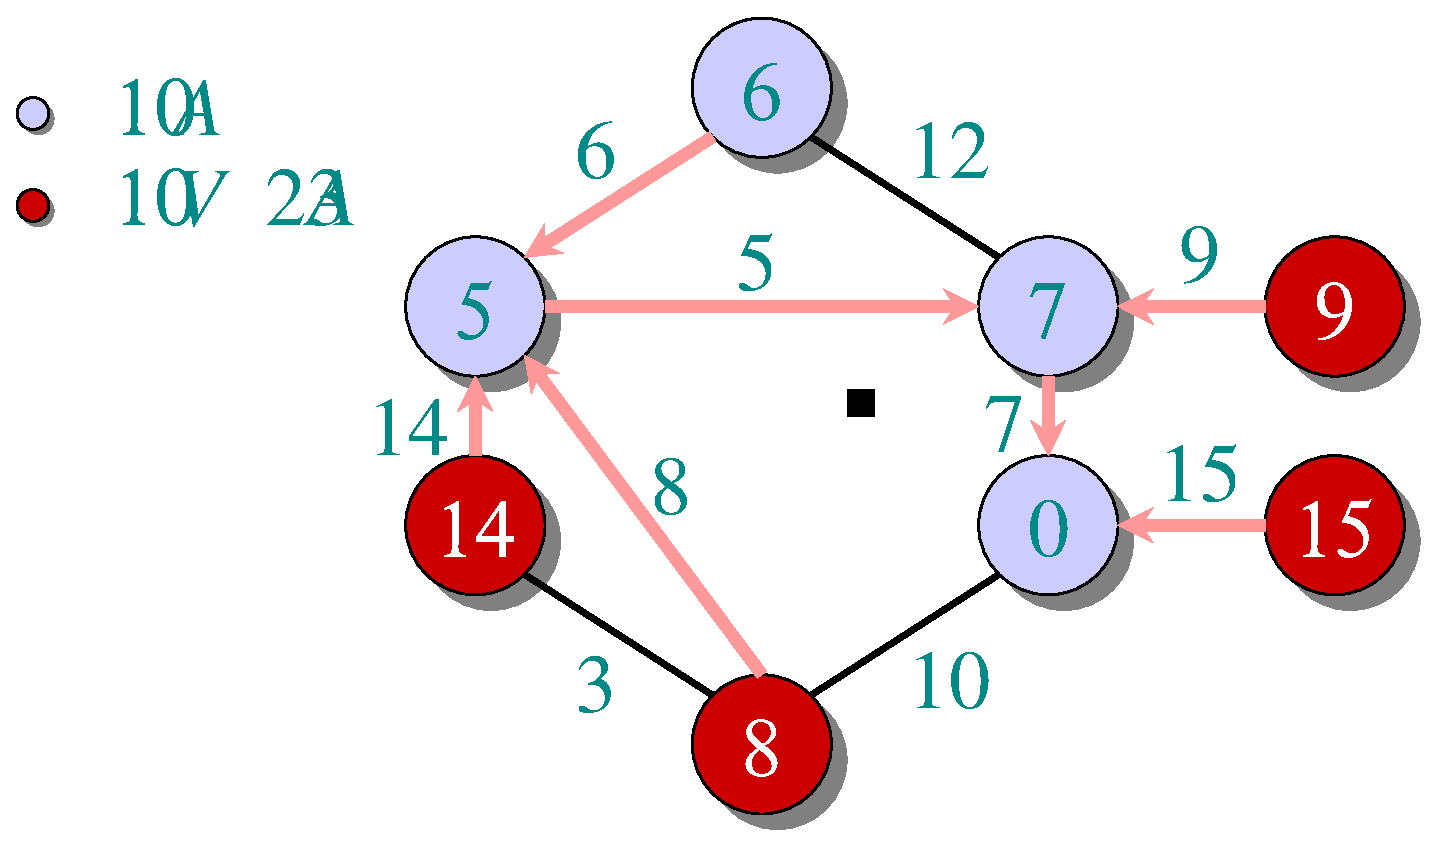
\includegraphics[width=4in]{lecture16/prim8.eps}
  \caption{Пример алгоритма Прима}
\end{figure}
\begin{figure}[ht]
  \centering
  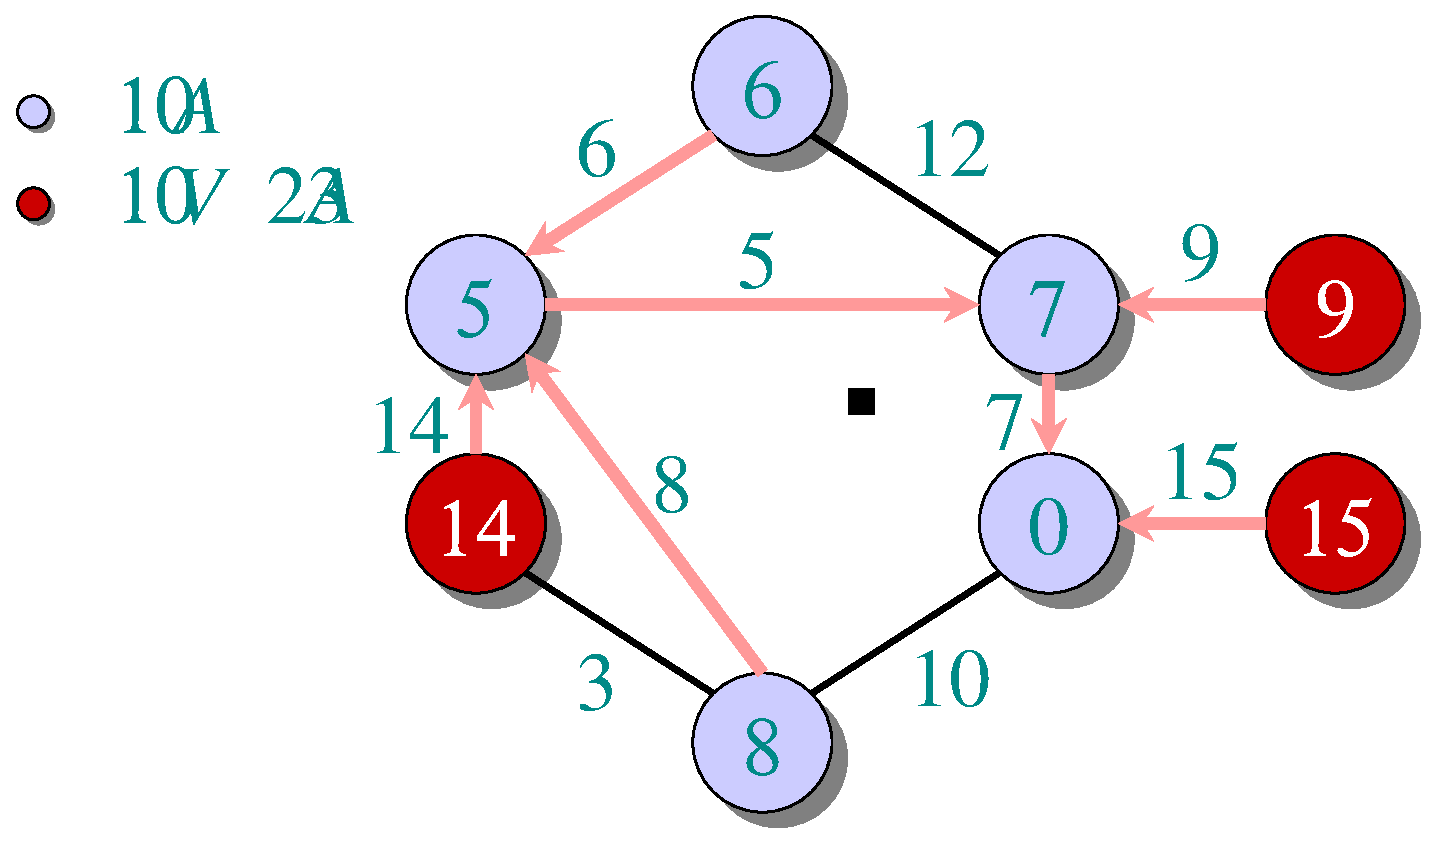
\includegraphics[width=4in]{lecture16/prim9.eps}
  \caption{Пример алгоритма Прима}
\end{figure}
\begin{figure}[ht]
  \centering
  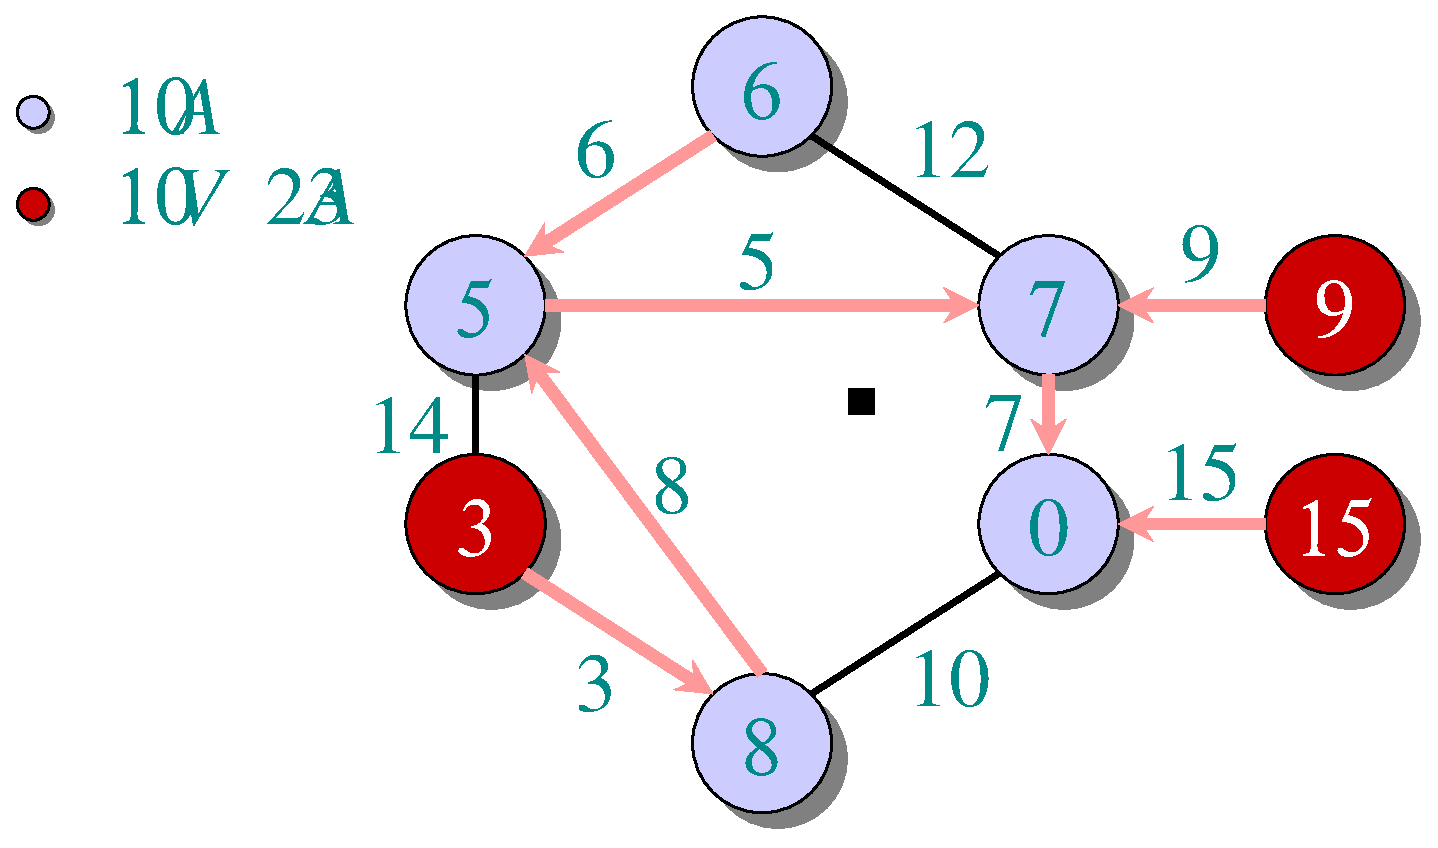
\includegraphics[width=4in]{lecture16/prim10.eps}
  \caption{Пример алгоритма Прима}
\end{figure}
\begin{figure}[ht]
  \centering
  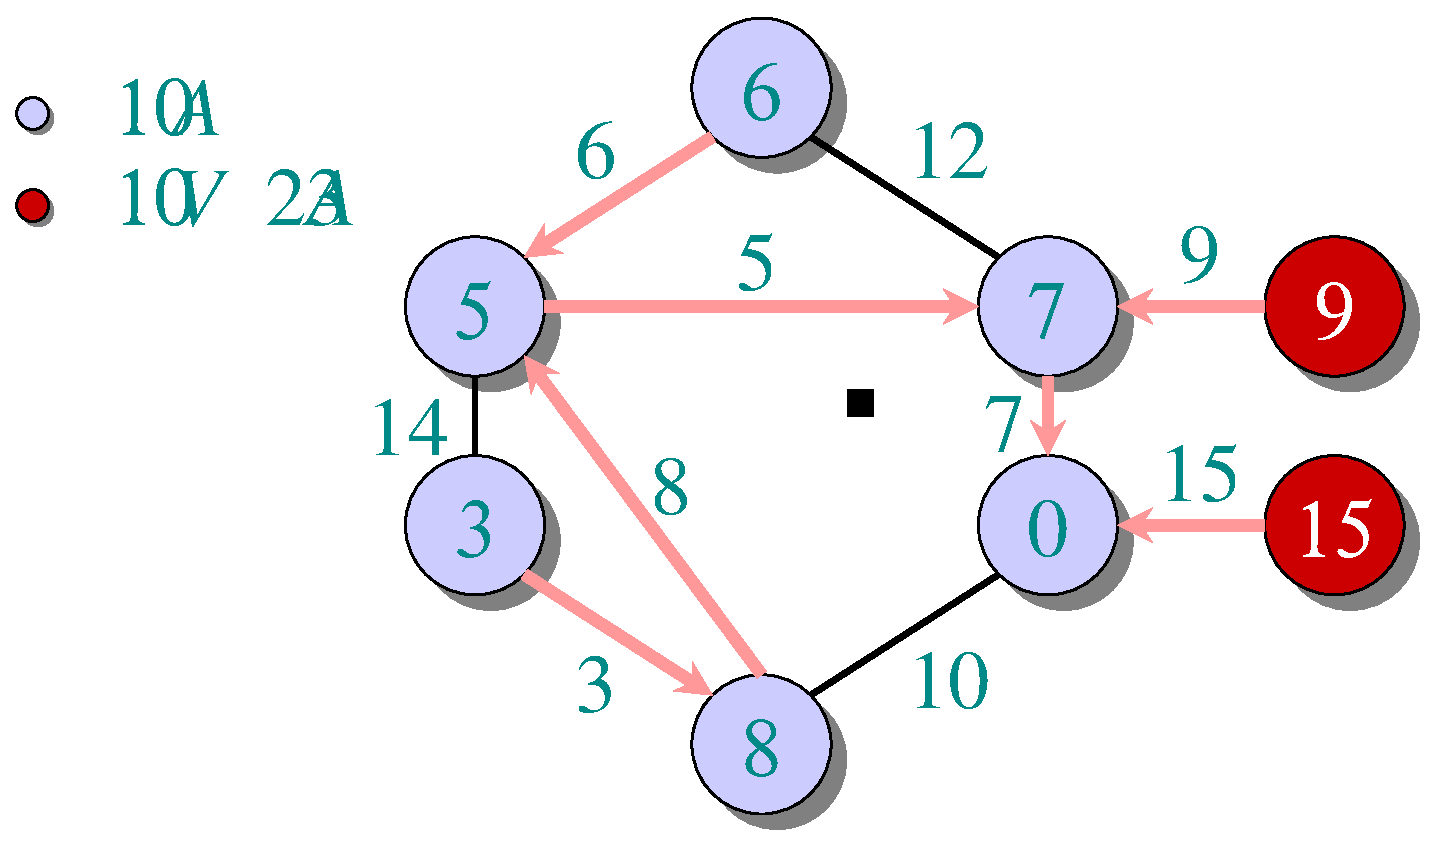
\includegraphics[width=4in]{lecture16/prim11.eps}
  \caption{Пример алгоритма Прима}
\end{figure}
\begin{figure}[ht]
  \centering
  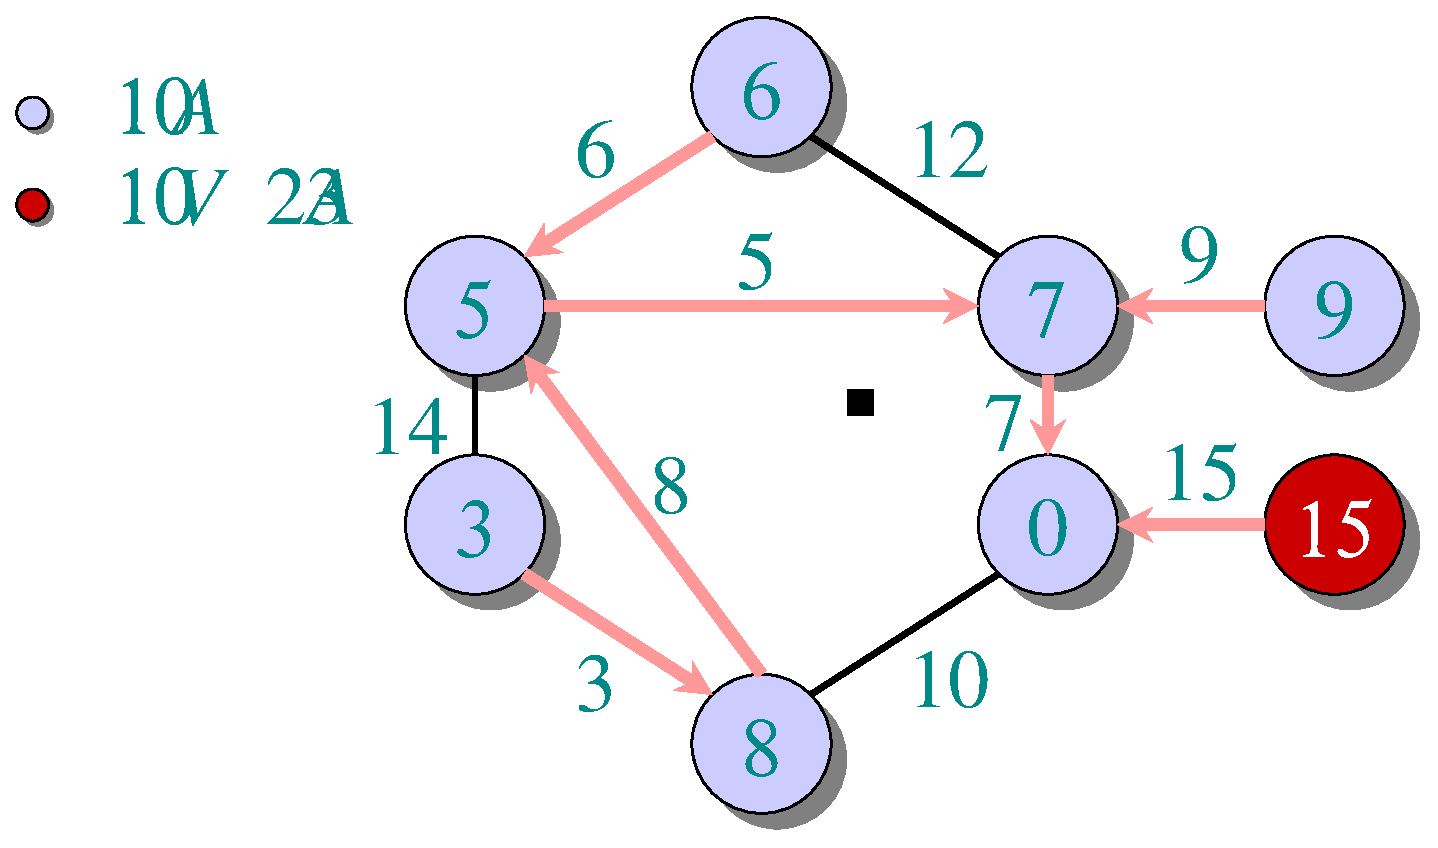
\includegraphics[width=4in]{lecture16/prim12.eps}
  \caption{Пример алгоритма Прима}
\end{figure}
\begin{figure}[ht]
  \centering
  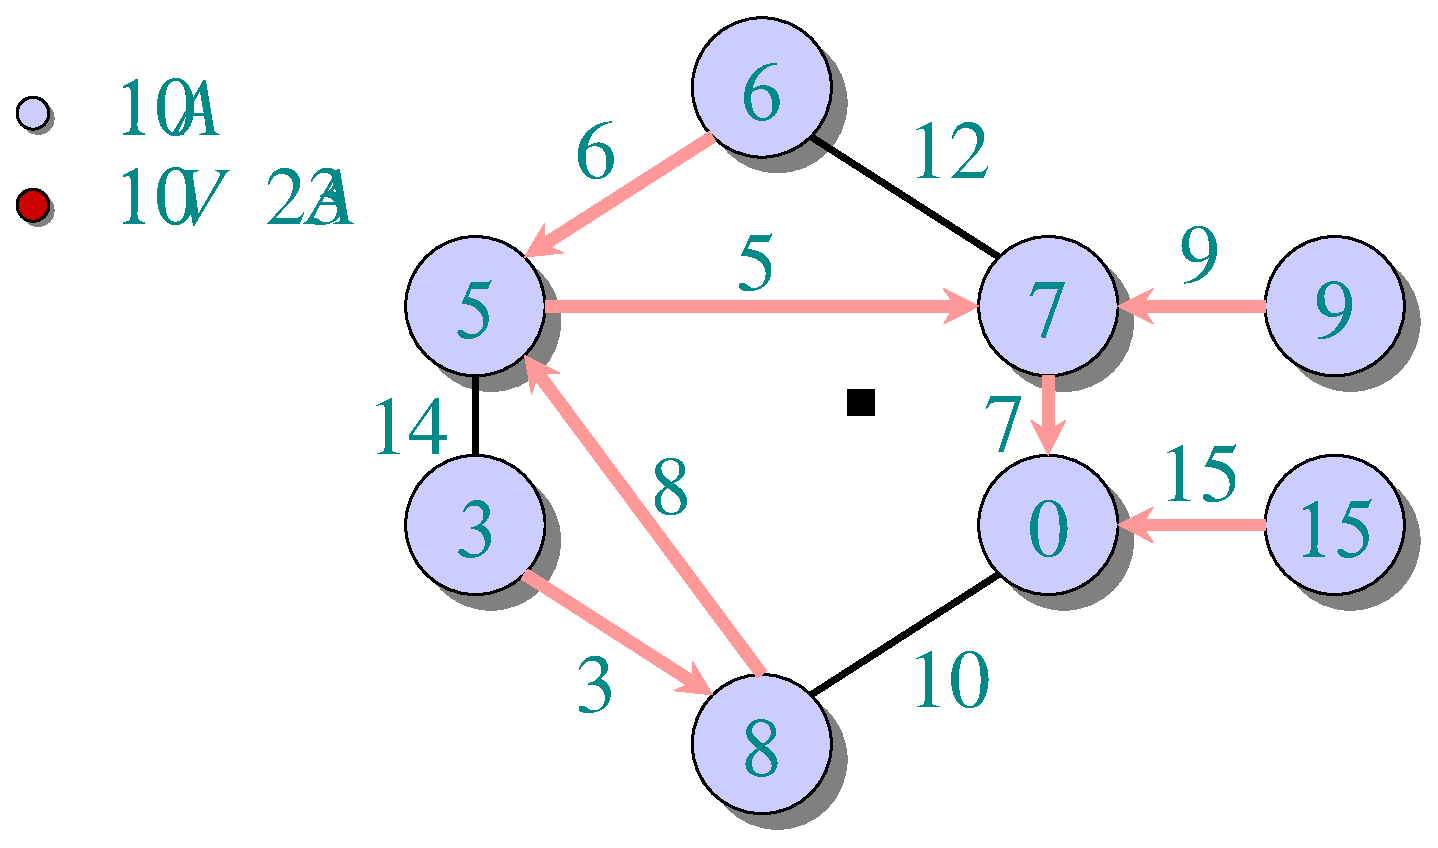
\includegraphics[width=4in]{lecture16/prim13.eps}
  \caption{Пример алгоритма Прима}
\end{figure}

Анализ алгоритма Прима

\begin{figure}[ht]
  \centering
  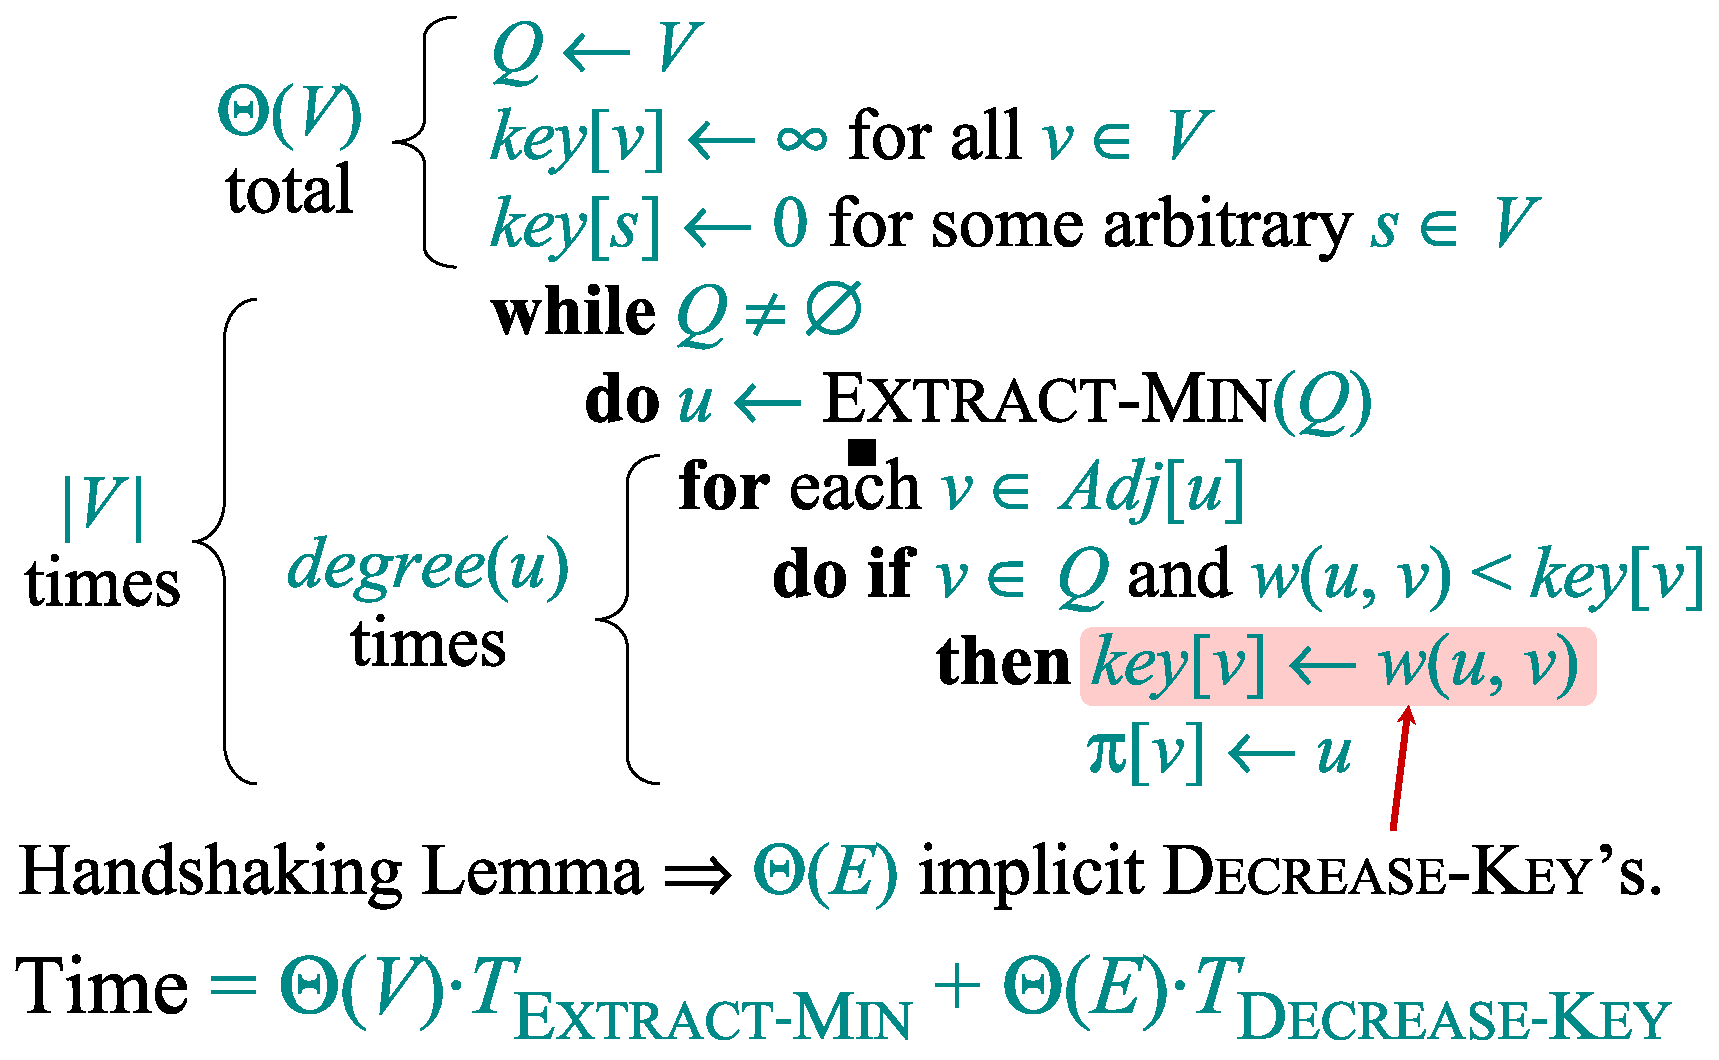
\includegraphics[width=4in]{lecture16/analysis.eps}
\end{figure}

\begin{figure}[ht]
  \centering
  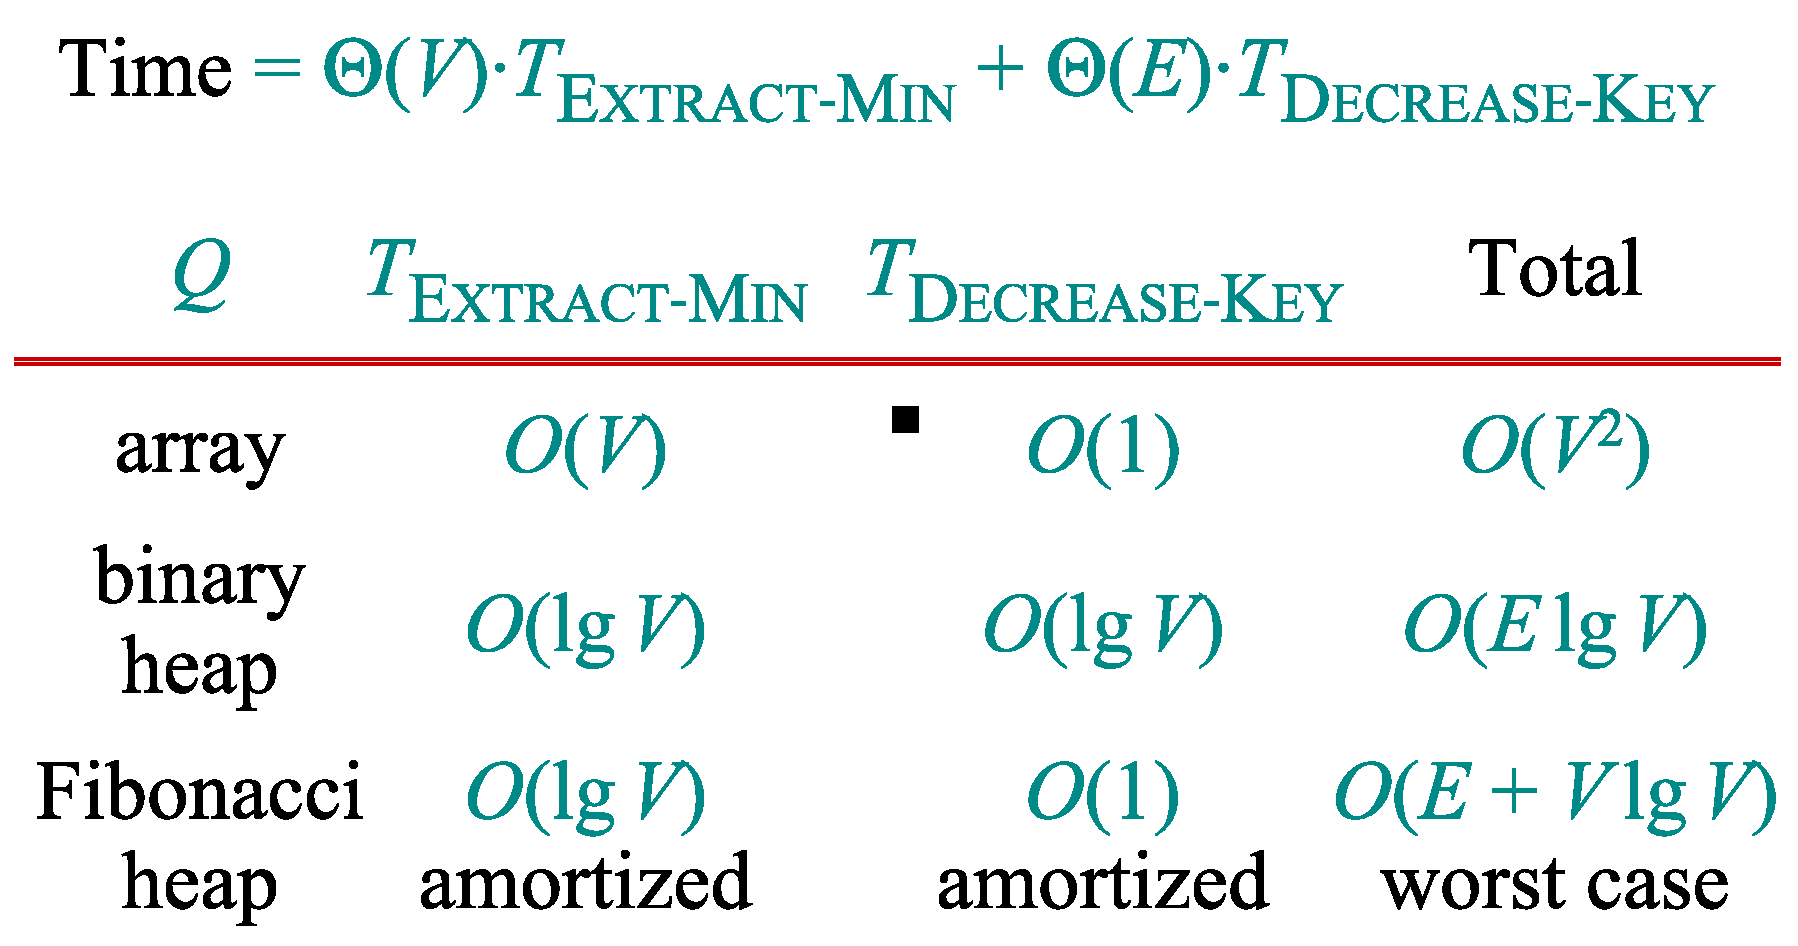
\includegraphics[width=4in]{lecture16/analysis2.eps}
\end{figure}

Другие алгоритмы для поиска МОД

\begin{itemize}
\item Алгоритм Крускала (с помощью непересекающихся множеств), время выполнения $O(E \lg V)$
\item Лучший известный на сегодня: рандомизированный алгоритма Каргера, Кляйна и
  Тарджана 1993го года, ожидаемое время выполнения = $O(V+E)$
  
\end{itemize}

\end{document}
